\documentclass[12pt]{article}
\usepackage{nopageno}
\usepackage{amsmath}
\usepackage{amssymb}
\usepackage[margin=0.5in]{geometry}
\usepackage{graphicx}
\usepackage{outlines}
\usepackage{hyperref}
\graphicspath{{./Images/}}
%When writing indented paragraphs:
%\usepackage{indentfirst}

\begin{document}
	\begin{center}
		% Header Image in ./Images/ folder
		% Source: extracted from https://web.northeastern.edu/ipl/wp-content/uploads/2017/09/IPL-Sample-Lab-Report.pdf
		
\includegraphics{Header}
		\vfill		
		\textbf{\Large{Report for Experiment \#N\\
		Lab Name}}
		\vfill
		Name\\
		Lab Partner: Name\\
		TA: Name\\
		Date
		\vfill
	\end{center}
	
	\section*{Abstract:}
		Summarize motivation and main results.
	
	\newpage
	
	\section*{Introduction:}
		\begin{outline}[enumerate]
			\1 State motivation – why you did this work?
			\1 Describe physics phenomena and methods of study.
			\1 Cover all investigations, keep short.
		\end{outline}
		Equations:
		\[ \vec{\nabla} \cdot \vec{E} = \frac{\rho}{\varepsilon_0} \tag{1} \]
		\[ \vec{\nabla} \cdot \vec{B} = 0 \tag{2} \]
		\[ \vec{\nabla} \times \vec{E} = - \frac{\partial \vec{B}}{\partial t} \tag{3} \]
		\[ \vec{\nabla} \times \vec{B} = \mu_0 \left( \vec{J} + \varepsilon_0 \frac{\partial \vec{E}}{\partial t} \right) \tag{4} \]
	
	\section*{Investigation n:}
		\begin{outline}[enumerate]
			\1 For each investigation: Discuss experimental set-up.
			\1 Explain experimental procedure.
			\1 Describe how the data was collected.
			\1 Include all data using graphs/tables, with titles.
				\2 If needed, include truncated raw data into Appendix.
				
		\begin{center}
			\begin{tabular}{c|ccc|c}
        			&            
        			& $\div q$    
         		&              
         		&        \\ \hline
         		& $ F = \kappa \frac{q_1 q_2}{r^2}$    
         		& $\rightarrow$ 
         		& $E = \kappa \frac{q}{r^2}$       
         		&        \\ $ \frac{d}{dx} $ 
         		& $\uparrow$ 
         		&               
         		& $\downarrow$ 
         		& $ \int dx$ \\
         		& $ U = \kappa \frac{q_1 q_2}{r}$    
         		& $\leftarrow$  
         		& $ V = \kappa \frac{q}{r}$      
         		&        \\ \hline
         		&            
         		& $ \times q $         
         		&              
         		&       
			\end{tabular}\\
			\begin{small} \textbf{
				Table n - Random Table (1)
			} \end{small}
		\end{center}
		
		\begin{center}
			% Plot Image in ./Image/ folder
			% Source: made with InkScape
			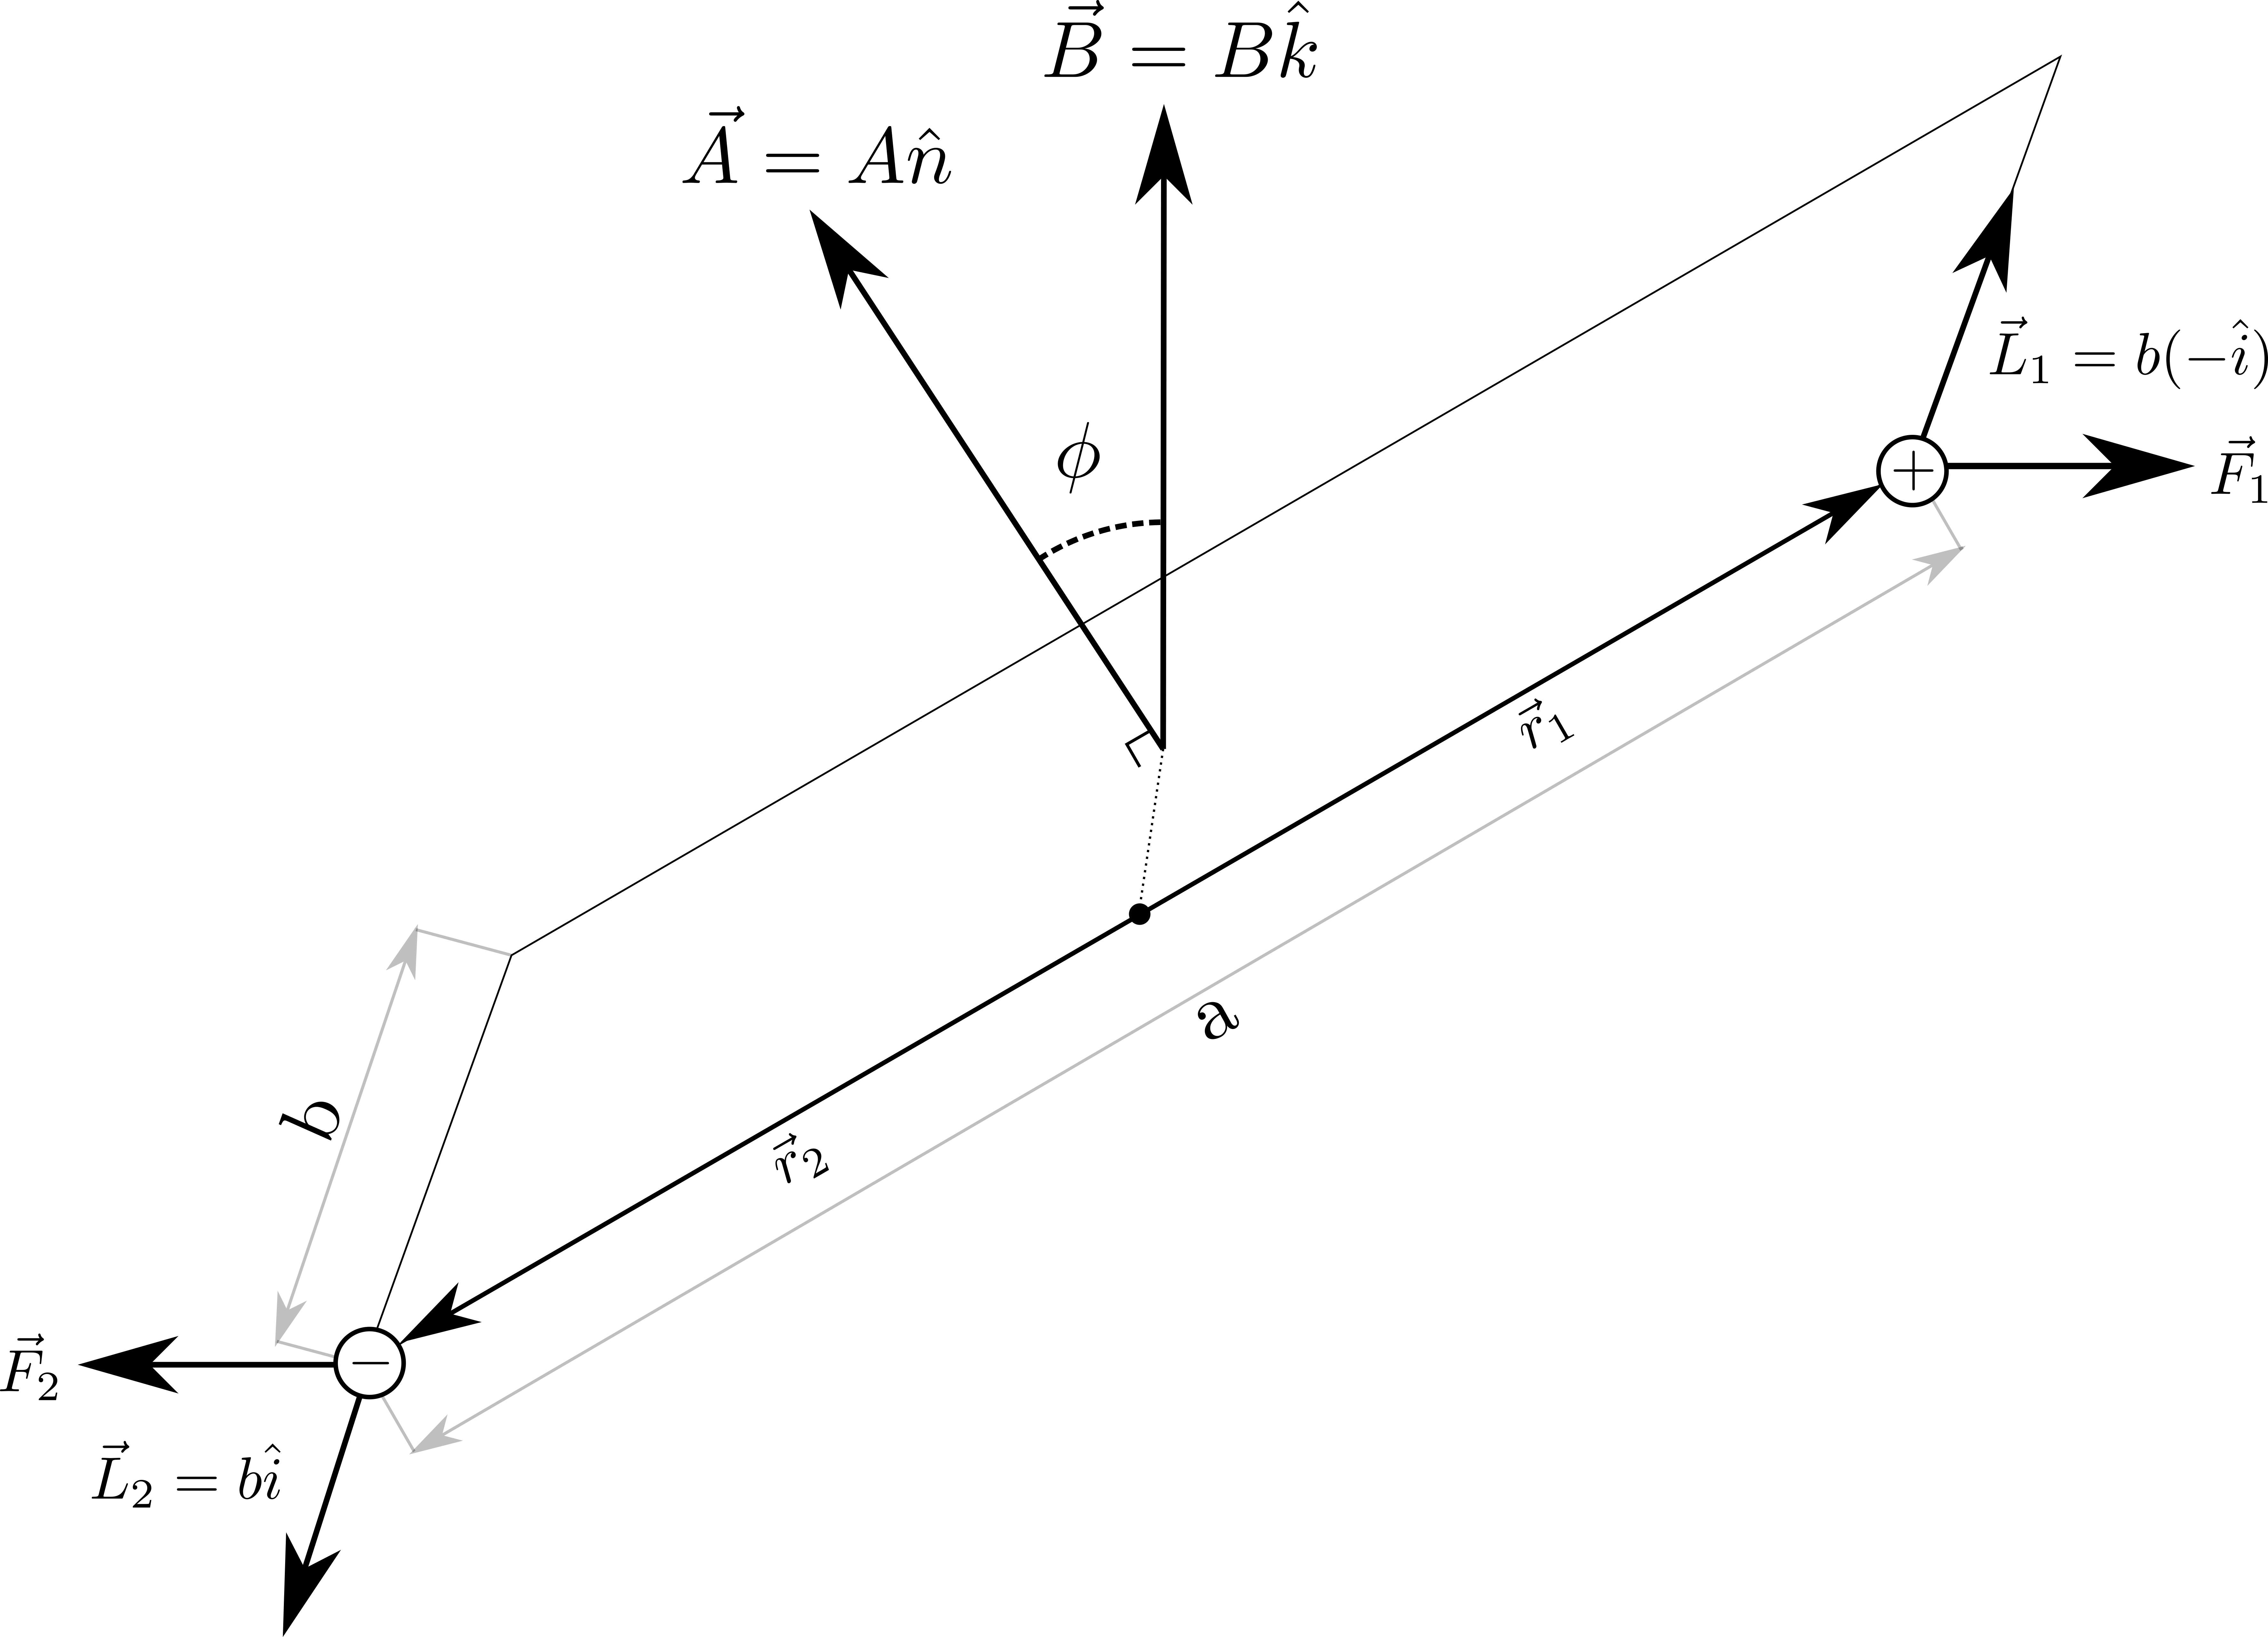
\includegraphics[width=4in]{RandFigure}\\
			\begin{small} \textbf{
				Figure n - Random Sample Figure
			} \end{small}
		\end{center}
				\2 Reference Table as [Table n], reference Figure as [Figure n]
			\1 Summarize physics concepts under investigation.
				\2 Cite equations as [1], [2], [3], [4] corresponding to tags in introduction.
			\1 Discuss relation between data and theory.
		 	\1 Describe techniques used to analyze data.
		 		\2 Cite references as (1), (2), (3), (4), corresponding to number in References.
		 	\1 Discuss sources/values of uncertainties in your measurement.
			\1 Write down main results with uncertainties.
			\1 Compare measured quantities to expected values.
			\1 Discuss if they match or not your expectations.
			\1 List the unaccounted factors in your analysis.
			\1 Argue why and how external factors may affect the results.\\
		\end{outline}
		
	\section*{Conclusion:}
		\begin{outline}[enumerate]
			\1 List physical concepts that have been investigated.
			\1 Summarize all main results that you obtained.
		 	\1 Discuss how external factors might have skewed the results.
			\1 Discuss possible improvements.
			\1 Keep to half a page.
		\end{outline}
		
	\section*{Questions:}
		\begin{outline}[enumerate]
			\1 Answer all questions at the end of experiment in the IPL Manual.
			\1 Type all necessary algebra, not just the answer.
			\1 Honors sections must answer extra question.
		\end{outline}
		
	\section*{References:}
		\begin{outline}[enumerate]
			\1 \href{https://www.tablesgenerator.com/#}{Table Generator \LaTeX}
			\1 \href{https://web.northeastern.edu/ipl/data-analysis/straight-line-fit/}{Northeastern IPL Straight Line Fit Calculator}
		\end{outline}
		
\end{document}